\section{High-Level Synthesis}
\label{bg:sec:high_level_synthesis}

\Acrfull{hls} is the process of compiling a high-level representation
of an application (usually in C, C++ or MATLAB) into a \gls{rtl}
implementation~\cite{coussy, gajski}.  In turn, this \gls{rtl} design
can be synthesized into a circuit and programmed onto the \gls{fpga}
device.  With modern \gls{hls} tools, some applications are synthesized
to have similar performance when compared with hand-crafted \gls{rtl}
implementations~\cite{bdti}.

The major advantage of \gls{hls} tools is that they enable us to work in a
\gls{hll}, as opposed to facing labour-intensive tasks such as optimizing
timing and designing control logic in the \gls{rtl} design process.  This
allows application designers to focus instead on the algorithmic and functional
aspects of their implementation~\cite{coussy}, without concerning themselves
with the intricate details of manual \gls{rtl} designs.

Another advantage of using \gls{hls} tools is that they are in general
more productive and less error-prone to work with, when compared with
traditional \gls{rtl} tools.  The reasons are two-fold.  Firstly, a C
description is smaller than a traditional \gls{rtl} description by a factor
of 10~\cite{coussy, bdti}.  Secondly, \gls{rtl} design can be notoriously
difficult to debug, whereas C code can be easily tested on an ordinary
microprocessor, and mature debug and analysis tools for C are freely
accessible~\cite{canis13}.

\Gls{hls} tools further benefit us in their ability to automatically search
the design space with a reasonable design cost~\cite{bdti}, potentially
exploring a large number of trade-offs between performance, cost and
power~\cite{mcfarland}.  Traditionally, this is generally much more difficult
to achieve in \gls{rtl} designs because of their low-level nature.

% Our thesis proposes a natural extension to HLS tools by automatically exploring
% the space of rewrites of floating-point numerical C programs, which are
% equivalent in real arithmetic, but could trade off accuracy, throughput and
% resource utilization when synthesized into circuits.

With recent advancements in this area, \gls{hls} tools have received a
resurgence of interest.  Many commercial tools have been released, such as
Catapult High-Level Synthesis~\cite{catapultc}, Impulse C~\cite{impulsec} and
PICO~\cite{schreiber02}, to meet the burgeoning demand from the \gls{fpga}
community.  Xilinx incorporates a sophisticated \gls{hls} flow for C/C++
named \gls{vhls} into its Vivado design suite~\cite{vivado_ds}, and their
SDAccel Development Environment~\cite{sdaccel} for C/C++/OpenCL allows data
centers to leverage \glspl{fpga}.  Altera's \gls{hls} solution is their Altera
SDC for OpenCL~\cite{aoc} which accelerates OpenCL applications on their
\gls{fpga} devices.  Besides commercial tools, many open-source \gls{hls}
tools have also been released in recent years, such as ROCCC~\cite{roccc},
Trident~\cite{tripp05} and LegUp~\cite{legup}.  LegUp is now gaining
significant traction in the research community.


\subsection{HLS Design Flow}
\label{bg:sub:hls_design}

This section provides an overview of the stages taken by the \gls{hls}
tool to compile a C program into \gls{rtl} implementation, by using
LegUp~\cite{legup, canis13} as our example.  LegUp is an \gls{hls} tool which
compiles programs to run on a hybrid software/hardware architecture, and its
design flow is shown in Figure~\ref{bg:fig:legup}, which consists of three
major stages to be explained below.
\begin{figure}[ht]
    \centering
    \includegraphics[width=0.7\linewidth]{bg/fig/legup}
    \caption{%
        The LegUp design flow, adapted from~\cite{canis13} and~\cite{legup}.
    }\label{bg:fig:legup}
\end{figure}

The first stage is to determine which parts of an application on the
function-level are suitable candidates to be synthesized into hardware
circuits, while the rest can be run on a soft-processor.  This stage starts
by compiling a C source program into a software executable targeting an
\gls{fpga}-based MIPS processor.  This processor has additional circuits
designed to profile the software implementation of the original application.
By running the compiled application on this processor, this profiling ability
allows the processor to use statistics such as number of clock cycles, power
and cache misses to identify problematic parts of the program at the function
level that will benefit from a hardware redesign, so that the power efficiency
and run time could be improved~\cite{canis13}.

After identifying functions of the application to be implemented as part of a
hardware architecture, the next stage is then to synthesize hardware designs
from these functions.  LegUp's synthesis toolchain is based on the \gls{llvm}
compiler infrastructure~\cite{llvm}, and it synthesizes C functions into
circuits in a series of steps.

It starts by using the \gls{llvm} front-end to compile a C function into
\gls{llvmir}, a platform-independent \gls{ir} that is capable of cleanly
representing \glspl{hll}~\cite{llvm_ir}, conventional and \gls{hls}-focused
compiler optimization passes are used to transform the \gls{ir} program, such
that the result when synthesized will have better performance when running on
the \gls{fpga}\@.

This is then followed by the \gls{hls} tool flow, which consists of four
logical steps: allocation, scheduling, binding and \gls{rtl} generation.  The
first step, \emph{allocation}, extracts information from the application and
user requirements to be used in subsequent stages, \eg~modules and \gls{ram}
blocks to be synthesized on the target device.  This is then followed by
\emph{scheduling}, which assigns the start and end states to each \gls{llvm}
instruction in a finite state machine~\cite{legup}, using a scheduling
algorithm based on the formulation of \gls{sdc}~\cite{legup, canis13, cong06}.
Many applications spend most of their time in loops; a scheduling technique
known as \emph{loop pipelining}, is therefore used in \gls{hls} tools to
make them run efficiently.  This technique admits greater parallelism by
allowing instructions in consecutive loop iterations to overlap as much as
possible.  LegUp uses \emph{modulo \gls{sdc} scheduling}~\cite{canis14}, which
we will cover in Section~\ref{bg:sub:sdc}, to minimize the wall-clock time
of a pipelined loop.  The third logical step, \emph{binding}, assigns each
operator in the program to functional units to be synthesized into hardware,
and maps program variables to registers.  The rationale behind this step is
that operators such as multipliers and dividers that tend to use a lot of
\glspl{lut} and \gls{dsp} blocks can be shared temporally.  Sharing these
functional units requires multiplexers, which is relatively expensive to
implement in \gls{fpga}\@.  Each assignment of an operator to a functional unit
is thus associated with a cost.  The problem of minimizing this cost is called
the assignment problem, which is efficiently solved in LegUp with a polynomial
time complexity using the Hungarian algorithm~\cite{canis13, kuhn10}.  Finally,
the \emph{\gls{rtl} generation} step gathers information produced from the
previous three steps, to generate Verilog source code corresponding to the C
function being compiled.

The third, and also the final stage, is to integrate software and
hardware components of the application into the \gls{fpga} device.
Following~\cite{canis13}, we explain it as follows.  Firstly, custom
accelerator circuits generated by \gls{hls}, a MIPS processor, and
communication interfaces between them are synthesized and programmed into the
\gls{fpga} device.  Because some of the functions in the original C source
code were implemented as hardware accelerators in the \gls{hls} compilation
flow, LegUp replaces them with wrapper functions which can invoke the hardware
accelerators in runtime.  Finally, this modified source code can then be
compiled into a MIPS binary to be executed on the \gls{fpga}\@.


\subsection{Loop Pipelining}
\label{bg:sub:pipelining}

Loop parallelism, and consequently, program run time is one of the main
optimization objectives we optimize later in Chapter~\ref{chp:latopt}.  Hence
in this subsection we first introduce the concept of loop pipelining.  We
consider our example program \verb|dotprod| in Figure~\ref{bg:lst:dotprod},
which computes the dot-product, \verb|d|, of two arrays \verb|A| and \verb|B|
of floating-point values.  We assume both arrays are stored in the same
\gls{ram}, which has one read port, and accessing this \gls{ram} has a one
cycle latency.  We further assume no limits on the number of arithmetic
operators that can by allocated, floating-point multipliers and adders are both
fully pipelined, and use $7$ and $10$ cycles respectively to produce outputs.
\begin{figure}[ht]
    \centering
    \begin{lstlisting}
    #define N 1024
    float dotprod(float A[N], float B[N]) {
        float d = 0.0f;
        for (int i = 0; i < N; i++) {
            d = d + A[i] * B[i];
        }
        return d;
    }
    \end{lstlisting}
    \caption{%
        A simple dot-product example which calculates the dot-product of two
        arrays \texttt{A} and \texttt{B}, each with 1024 elements.
    }\label{bg:lst:dotprod}
\end{figure}

A trivial way to schedule the loop in \verb|dotprod| is to allow each iteration
to complete before starting the next iteration; this is however not very
efficient.  As we can see in Figure~\ref{bg:fig:schedule}, with a good
schedule, operations across loop iterations can often temporally overlap,
giving way to parallelism and improve performance of the loop execution.  In
Figure~\ref{bg:fig:schedule}, iterations are laid out in rows, each clock cycle
is a column, \textbf{mul} and \textbf{add} are multiplication and addition
respectively, \verb|A[0]| and \verb|B[0]| are read accesses from the two
arrays, and the arrows indicate the data-flow of \verb|d| across iterations.
This schedule allows consecutive iterations to start every 10 cycles; and this
number of clock cycles between the start of consecutive iterations is known
as the \gls{ii}\@.  Loop iterations in this schedule repeat for $1024$ times
(the \emph{trip count}, $N$), and each iteration requires $19$ cycles (the
\emph{depth}, $D$, of the loop), as a result the overall latency $L$ of this
loop is $(N - 1) \times \II + D = (1024 - 1) \times 10 + 19 = 10,249$ cycles.
\begin{figure}[ht]
    \centering
    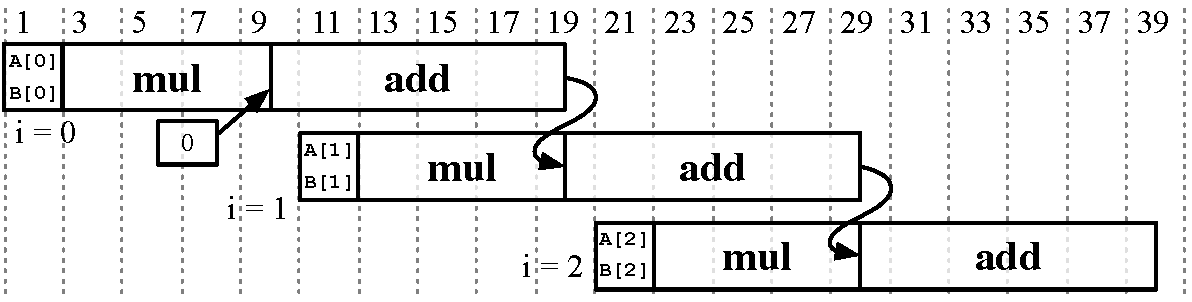
\includegraphics[width=0.8\linewidth]{bg/fig/schedule}
    \caption{%
        The resulting schedule of the example program in generated.
    }\label{bg:fig:schedule}
\end{figure}

Any valid schedule of this loop must satisfy the constraints imposed by
data-dependences.  For instance in our example, it is clear that in a
\emph{single} iteration, in the loop body, multiplication of \verb|A[i]|
and \verb|B[i]| must precede addition of \verb|d| and the multiplied
result.  Furthermore, in the $(i + 1)$-th iteration, access to the variable
\verb|d| must wait until \verb|d| is updated with a new value in the $i$-th
iteration, data-dependences therefore also exist on \verb|d| \emph{across}
loop iterations.  We call the former kind of dependences \emph{intra-iteration
dependences} and the latter \emph{inter-iteration dependences}.

Besides data-dependence constraints, the number of resources available also
affects loop scheduling.  For instance, under our assumption in \verb|dotprod|
the \gls{ram} can only be read once per cycle, our schedule thus should avoid
reading from the same \gls{ram} in the same clock cycle.  We say a schedule is
optimal, in the sense that the overall latency $L = (N - 1) \times \II + D$,
is minimized, while none of the constraints are violated.  However with a much
more complex program, finding the optimal schedule is often an intractable
task.  Limits on resource availability, along with dependence constraints,
make scheduling an NP-hard problem which is difficult to solve optimally and
efficiently~\cite{hwang91}.  In the following part of this section, we discuss
modulo \gls{sdc} scheduling~\cite{zhang13, canis14} used in \gls{hls} tools,
such as LegUp, to efficiently attack the scheduling problem.


\subsection{Modulo SDC Scheduling}
\label{bg:sub:sdc}

Many algorithms exist to schedule pipelined loops.  For example,
Fan~\etal~\cite{fan08} proposed that a schedule can be found by formulating
the constraints into a \gls{smt} problem and use an \gls{smt} solver to modulo
schedule operations.  An alternative technique, \gls{ims}~\cite{rau94}, has
been a widely adopted by compilers that use software pipelining to schedule
instructions for \gls{vliw} processors~\cite{mcnairy03}.  This method has also
been widely adopted in \gls{hls} tools such as PICO-NPA~\cite{schreiber02},
Trident~\cite{tripp05} and LegUp~\cite{canis13, canis14}.  \Gls{ims} for
software pipelining~\cite{rau94}, however did not consider operator chaining,
\ie~allowing operations with combinational logics in a data-flow sequence to
be carried out in the same clock cycle.  Schreiber~\etal~\cite{schreiber02}
in their adoption of \gls{ims} in \gls{hls}, found operator chaining
to be non-trivial in \gls{ims} and requires static timing analysis of
combinational components~\cite{canis14}.  A new method, the modulo \gls{sdc}
scheduling algorithm, has thus recently gained traction and has been
used by Canis~\etal~\cite{canis14} in their LegUp and by Zhang~\etal{}
in~\cite{zhang13}, because an \gls{sdc} formulation is more suited to model
the effect of chaining operators.  For this reason, an overview of the modulo
\gls{sdc} scheduling approach is provided in this subsection.

\subsubsection{Constructing the Data-Dependence Graph}

In the first stage of modulo \gls{sdc} scheduling, dependence relations are
extracted from the body of this loop.  These dependence relations form a
dependence graph, where vertices are operations, and edges between pairs of
vertices indicate dependence relations.  This dependence graph can subsequently
be used to derive data-dependence constraints.  Figure~\ref{bg:fig:depgraph}
shows the complete dependence graph of \verb|dotprod|'s loop body.
\begin{figure}[ht]
    \centering
    \begin{tikzpicture}
        \node (ai)  at (0,0) {\texttt{A[i]}};
        \node (bi)  [right=of ai, xshift=5mm] {\texttt{B[i]}};
        \node (mul) [below right=of ai, xshift=-5mm, yshift=5mm]
            {$\times$};
        \node (sum) [left=of mul, xshift=-10mm] {\texttt{d}};
        \node (add) [below right=of sum, xshift=-4mm, yshift=5mm] {$+$};
        \draw[->] (ai)  -- node[auto]{\smallpair10} (mul);
        \draw[->] (bi)  -- node[auto]{\smallpair10} (mul);
        \draw[->] (mul) -- node[auto]{\smallpair70} (add);
        \draw[->] (sum) -- node[auto]{\smallpair00} (add);
        \draw[->,dashed]
            (add) to[out=-135, in=180] node[left=3pt]{\smallpair{10}{1}} (sum);
    \end{tikzpicture}
    \caption{%
        The dependence graph formed by the data-dependences in the loop body
        of the dot-product example in Figure~\ref{bg:lst:dotprod}.  The dashed
        edge highlights the inter-iteration dependence.
    }\label{bg:fig:depgraph}
\end{figure}

Intra-iteration dependence edges in the graph are each labelled with $\langle
l, 0 \rangle$, a pair of attributes of integers accordingly.  The first integer
$l$ signifies the number of clock cycles that must elapse between the start of
the predecessor and the successor operations.  The latter value $0$ indicates
that the dependence occurs in the same iteration.  To illustrate, the edge
between the multiplier ``$\times$'' and adder ``$+$'' has an attribute $\langle
7, 0 \rangle$, because ``$\times$'' takes 7 cycles to generate an output.

Additionally, inter-iteration dependences create elementary cycles in the
dependence graph.  For example, in each iteration the initial value of \verb|d|
depends on the final value of \verb|d| from the previous iteration.  In this
graph we thus add an edge from the output of the addition to the variable
\verb|d|.  We further describe that this dependence has a \emph{dependence
distance} of $1$, as $1$ iteration must elapse between the start of each pair
of value updates and its corresponding use.  This edge is then assigned
an attribute $\langle 10, 1 \rangle$ which signifies that the adder has a
latency of $10$ cycles, and this dependence has a distance $1$.

\subsubsection{Finding the Minimum Initiation Interval}

Modulo \gls{sdc} scheduling owes its efficiency to assuming an initial
constant \gls{ii} and attempting to search for a schedule that satisfies all
constraints.  This search stops if a feasible schedule is found, otherwise
\gls{ii} can be incremented by 1 and the search is repeated until we discover
a valid schedule.  To begin, we can find a lower bound on \gls{ii}, which we
call the \gls{mii}, as our initial constant \gls{ii}\@.  The \gls{mii} is
computed such that all schedules with an \gls{ii} less than \gls{mii} violate
some constraints.  For each of the inter-iteration dependences and resource
constraints, an \gls{mii} can be found, respectively known as \gls{recmii} and
\gls{resmii}~\cite{rau94, canis14, zhang13}.  We first introduce methods to
compute both values, then the overall \gls{mii} can then be computed using the
following equation:
\begin{equation}
    \MII = \max\left(\RecMII, \ResMII\right).
\end{equation}

Firstly, we compute \gls{resmii}, by finding the most constrained resources
in the loop, as these limits impact the \gls{resmii} value.  For example,
\verb|dotprod| does not impose limits on the number of floating-point operators
that can be allocated, but assumes there is a constraint which restricts the
rate of memory accesses, \ie~only one read is allowed in each clock cycle.
Because each iteration requires two accesses to the same memory, a $\ResMII =
2$ will thus fully occupy the \gls{ram} throughput.  To generalize this to all
loops, we consider for each type of operation $\opsymbol$ being used in the
loop, the number of available resources $r_\opsymbol$ for $\opsymbol$ and the
number of occurrences $n_\opsymbol(G)$ of $\opsymbol$ in the loop dependence
graph $G$, to evaluate $\left\lceil n_\opsymbol(G) / r_\opsymbol \right\rceil$,
the maximum ratio constitutes the final \gls{resmii}, or equivalently:
\begin{equation}
    \ResMII = \max_{\opsymbol~\in~\mathrm{OpTypes}}
        \left\lceil
            \frac{n_\opsymbol(G)}{r_\opsymbol}
        \right\rceil,
\end{equation}
where $\mathrm{OpTypes}$ is the set of all types of operations, \eg~array
accesses, arithmetic units, and others, used in the loop.

The second step is to evaluate a minimal \gls{recmii} by ensuring for all
cycles $c$ in the graph $G$ the following inequalities hold:
\begin{equation}
    \forall c \in \mathrm{Cycles}(G):
        \sum_{e \in c} \mathrm{lat}(e) - \RecMII \times
        \sum_{e \in c} \mathrm{dist}(e) \leq 0,
\end{equation}
where $\mathrm{Cycles}(G)$ computes the set of all cycles in the graph $G$;
$e \in c$ enumerates all edges in the cycle $c$; and for an edge $e$ between
two vertices $v_1$ and $v_2$ of the form $v_1 \xrightarrow{\langle l, d
\rangle} v_2$, $\mathrm{dist}(e)$ and $\mathrm{lat}(e)$ respectively evaluate
to the latency $l$ and dependence distance $d$.  Hence, $\sum_{e \in c}
\mathrm{lat}(e)$ and $\sum_{e \in c} \mathrm{dist}(e)$ respectively sum
the latencies and dependence distances along all edges in the cycle $c$.
Equivalently, we can derive an equation for \gls{recmii} for the graph $G$:
\begin{equation}
    \RecMII = \max_{c~\in~\mathrm{Cycles}(G)}
        \left\lceil \frac{%
            \sum_{e \in c} \mathrm{lat}(e)
        }{%
            \sum_{e \in c} \mathrm{dist}(e)
        }
        \right\rceil.
\end{equation}
For example, in the dependence graph (Figure~\ref{bg:fig:depgraph}) of our
simple program (Figure~\ref{bg:lst:dotprod}), one cycle,
\tikz[baseline=-0.65ex]{%
    \node(d) at (0, 0) {\texttt{d}};
    \node(plus) at (5ex, 0) {$+$};
    \draw[->] (d)-- (plus);
    \draw[->,dashed] (plus) to[out=115, in=65] (d);
},
exists and the sums of latencies and dependence distances along this cycle are
$10$ and $1$ respectively, thus the \gls{recmii} of this graph is $\lceil 10 /
1 \rceil = 10$.

The simplest possible method of finding \gls{recmii} is therefore to enumerate
all cycles in the graph and compute the ratio between sums of latencies
and dependence distances.  Unfortunately in the worst case, the number of
cycles is exponential in the number of edges in a graph, this approach could
become intractable for large loops.  An alternative method based on the
Floyd-Warshall shortest path algorithm~\cite{floyd62} which runs in polynomial
time, is thus proposed in~\cite{rau94} to efficiently find \gls{recmii}.

\subsubsection{Scheduling Operations}

After assuming a tentative constant \gls{ii}, in modulo \gls{sdc} scheduling,
we try to construct an \gls{sdc} problem in order to solve for the schedule.
We aim to assign each operation, corresponding to each vertex $v$ in the graph,
to a time slot $s_v$ when it begins its operation.  While in this process, the
scheduling must ensure that no assignment violates data-dependence and resource
constraints.  For instance if a multiply operation is allocated with a time
slot in the second clock cycle, in each iteration it will start computation in
the second clock cycle of that iteration.

To begin, we ignore the resource limits for now and formulate an \gls{sdc}
problem for the dependence constraints.  For each dependence edge $u
\xrightarrow{\langle l, d \rangle} v$ from vertex $u$ to vertex $v$ in the
graph, it is possible to write down the following inequality, where $s_u$ and
$s_v$ are respectively the time slots for vertices $u$ and $v$:
\begin{equation}
    s_u - s_v \leq \II \times d - l.
\end{equation}
For instance, the edge $\times \xrightarrow{\langle 7, 0 \rangle} +$ is an
intra-iteration dependence, hence \gls{ii} does not constraint the scheduling
relation between these two operations and we substitute $d$ with $0$ and $l$
with $7$, and the \gls{ii} term vanishes, to derive~\eqref{bg:eq:sdc_intra}
below, and the back-edge $+ \xrightarrow{\langle 10, 1 \rangle} \mathtt{d}$
produces the following inequality in~\eqref{bg:eq:sdc_inter}:
\begin{align}
    s_\times - s_+ &\leq -7,
    \label{bg:eq:sdc_intra} \\
    s_+ - s_\mathtt{d} &\leq \II - 10.
    \label{bg:eq:sdc_inter}
\end{align}

Besides dependence constraints, additional constraints are used to limit the
length of critical paths in combinational logics, such that for instance, a
long chain of additions can be broken down into multiple cycles to guarantee
the frequency requirement.  For all paths $u \rightarrow \cdots \rightarrow
v$ between inter-iteration dependent vertices $u$ and $v$ consisting of
only combinational logics, it is possible to compute a critical path delay
$\mathrm{delay}(u, v)$.  This critical path delay is defined as the largest sum
of propagation delays of each intermediate operation along any combinational
path from $u$ to $v$.  For a pair of dependent vertices $u$ and $v$ such
that $\mathrm{delay}(u, v) > T_\mathrm{clk}$, where $T_\mathrm{clk} =
\frac{1}{f_\mathrm{clk}}$ and $f_\mathrm{clk}$ is the target clock frequency,
we can create the following constraint~\cite{cong06}:
\begin{equation}
    s_u - s_v \leq - \left\lceil
        \frac{
            \mathrm{delay}(u, v)
        }{
            T_\mathrm{clk}
        }
    \right\rceil + 1.
\end{equation}
This inequality ensures that for any the critical path delay between $u$
and $v$ greater than $T_\mathrm{clk}$, this path cannot be scheduled within
one clock cycle and it should be split into at least $ \left\lceil \frac{
\mathrm{delay}(u, v) }{ T_\mathrm{clk} } \right\rceil $ cycles.

Besides dependence and frequency constraints, Zhang~\etal~\cite{zhang13}
further introduces optional ones, such as lifetime constraints, which aim to
minimize the register requirements, and relative timing constraints, which can
be used to satisfy the timing requirement of user-specified I/O protocols.

The rationale of using the \gls{sdc} formulation to model constraints
is that the feasibility of an \gls{sdc} system and the corresponding
solution, if it exists, can be found efficiently.  More precisely, using the
Bellman-Ford algorithm~\cite{schrijver05}, it can run in $\Theta(l n)$ time,
where $l$ is the number of constraint inequalities and $n$ is the number
of variables~\cite{zhang13}.  Additionally, an \gls{sdc} problem can be
incrementally solved, \ie~a new solution, if exists, can be updated in $\bigo(m
+ n \log n)$ time when a constraint is added or removed, by using the algorithm
presented by Ramalingam~\etal~\cite{ramalingam99}.  In contrast, traditional
\gls{ilp} scheduling techniques make use of $\bigo(mn)$ variables to represent
a scheduling problem, where $m$ is the number of time slots and $n$ is the
number of operations~\cite{hwang91}, and solving this \gls{ilp} problem often
demands expensive branch-and-bound procedures~\cite{zhang13} as \gls{ilp} is
NP-complete~\cite{karp10}.

Unfortunately, resources constraints, because of their non-linearity, cannot
be easily expressed as \gls{sdc} constraints.  Therefore, a data structure
called the \gls{mrt} is used to keep track of resource constraints as the loop
is incrementally scheduled~\cite{canis14}.  The \gls{mrt} has \gls{ii} columns
and each row tracks an available resource.  When a certain resource is used in
the time slot $s_u$, the \gls{mrt} records an entry for this resource in column
$s_u \mod \II$ and the corresponding row of this resource.  To illustrate,
consider our example in Figure~\ref{bg:lst:dotprod}, which assumes a single
read to the memory in one cycle for both arrays.  The \gls{mrt} thus has $\II =
10$ columns, and $1$ row for accessing the memory.  If \verb|A[i]| is assigned
with a time slot $0$, then a schedule assigning \verb|B[i]| to the same time
slot must be invalid, because a record exists for \verb|A[i]| in row $1$ column
$0$, and thus \verb|B[i]|, which is competing for the same resource, hence must
be scheduled in a later time slot.

A typical modulo \gls{sdc} scheduling algorithm begins with a schedule
without resource constraints.  A priority function is then used to sort
all resource-constrained operations by perturbation, \ie~we place greater
importance to operations that have a larger impact on the schedule when they
are moved~\cite{canis14}.  For each operator $u$ in this sorted list, if $u$ is
currently scheduled at time slot $t_u$ and does not have a resource conflict
in the \gls{mrt}, a new constraint $s_u = t_u$ is constructed, otherwise a
different constraint $s_u \geq t_u + 1$ is used to ensure the operation $u$
is scheduled at least one cycle later, so that it does not compete for the
resource in time slot $t_u$.  This newly created constraint is then tentatively
added to the \gls{sdc} problem.  For a feasible resulting \gls{sdc} problem,
a new solution can be found incrementally, otherwise the algorithm backtracks
to a latest feasible \gls{sdc} formulation and try to schedule other operators
before $u$.  A time budget can also be used to limit the number of attempts to
schedule resource-constrained operators; if a valid schedule cannot be found
under the given budget, the \gls{ii} can be incremented by $1$ to relax the
dependence and resource constraints, and the above mentioned procedure can be
repeated until a valid schedule is found.


\subsection{Obstacles in Adoption}
\label{bg:sub:obstacles_in_adoption}

High-level synthesis, with its development-cost advantage over traditional
\gls{rtl} design paradigm, is gaining traction in the circuit design community.
It is however in its early phase, and these tools still pose challenges in
terms of using them as early adopters.

\Gls{hls} tools may have limited support for \gls{hll} constructs.  For
instance, \gls{vhls} requires pointer arrays to reference values or arrays of
values, platform-specific functions such as \verb|memcpy()| and \verb|memset()|
are supported but \verb|const| values must be used, and finally, while
tail-recursive functions written with C++ template constructs can be
transformed into loops in compile time, recursion in general cannot be
implemented~\cite{vivado_hls}.  Additionally, software programs often rely
on libraries, many of which are platform-specific, whereas in \gls{hls}\@,
these libraries may not be appropriate and may likely be unavailable.  These
above limitations make migrating existing software source code to a functional
\gls{hls} design a demanding task.

Optimizing C code for \gls{hls} could be a laborious process and requires
expertise in hardware design.  Although software compilers face similar
challenges to make programs run faster, experienced programmers can often
manually fine-tune software implementations for performance.  Because of
the flexibility of \glspl{hll}, currently it is difficult for designers
to apply common intuitions, and the quality of the synthesis result may
be difficult to predict~\cite{gupta04}.  Winterstein~\etal~\cite{felix13}
implemented K-means clustering algorithms in \gls{hls}, and discovered that
with extensive manual code transformations and \verb|#pragma| statements
that are specific to \gls{vhls}, the tool can be persuaded to produce an
efficient circuit.  When compared to the \gls{rtl} counterparts, their
\gls{hls} designs achieved up to 40\% of the performance in terms of area-time
product.  Zhang~\etal~\cite{zhang15} implemented a \gls{cnn} accelerator in
\gls{vhls}, they optimized their design by program transformations techniques
such as loop interchange, tiling, pipelining and unrolling, and noticed that
by enumerating combinations of loop tile sizes, loop nest ordering and unroll
factors, they were able to select the best implementation by analytically
estimating the throughput of each.  Similarly, Suda~\etal~\cite{suda16}
explored the design space of their \gls{cnn} accelerator by solving a
resource-constrained throughput optimization problem, in order to generate
a high-performance \gls{cnn} accelerator to be synthesized in Altera OpenCL
compiler~\cite{aoc}.  \Gls{hls} tools can provide some syntactic constructs
to automate lower-level code transformations such as instruction parallelism,
loop pipelining and unrolling.  It is however up to the engineer to decide how
to utilize these transformations, and to determine whether they will improve
the design.  Higher-level optimizations such as the manual design space
exploration explained in earlier examples, may allow tools to vastly improve
the performance of \gls{hls} applications.  Automating these techniques in
\gls{hls}, however, remains a significant challenge.

\Gls{hls} tools can often make use techniques such as loop pipelining
discussed in Section~\ref{bg:sub:sdc} to detect and exploit parallelism at the
instruction-level.  Coarser-grain parallelism, which is tightly associated
with the algorithmic details, is however much more complex~\cite{nane15}, and
many optimization opportunities are not yet exploited by \gls{hls} tools.  For
instance, unlike the \gls{cpu}, which has a monolithic storage and thus their
performance is often limited by the memory wall, the \gls{fpga} has dedicated
\gls{ram} blocks in the logic fabric to distribute memory bandwidth via data
reuse. \glspl{hll} such as C were designed with a mindset of the von Neumann
architecture, and the source code in C typically does not specify how the
memory hardware is utilized.  For this reason, \gls{hls} tools must be able to
intelligently partition a monolithic memory into smaller chunks that can be
accessed in parallel, in order to maximize performance; how to attain this is
still a challenging research area~\cite{cong11, cong12, wang13, felix15}.

Circuits produced by \gls{hls} tools are expected to be semantics-preserving.
This means that they should be functionally equivalent to the original
C programs; in other words, for any given program inputs, the tools
should guarantee that the computed outputs from the original C code
and the synthesized circuit should be identical.  A different class of
optimizations, which we call \emph{lossy optimization}, break this promise by
optimizing data-paths in a way that may impact numerical accuracy.  \Gls{hls}
tools could benefit from these optimizations in the future, which bring
further performance improvements that cannot be attained by traditional
optimizations alone.  Because these approaches could affect numerical
accuracy, performance optimization and round-off error analysis may be
carried out simultaneously.  We will further discuss lossy optimization
methods such as expression balancing enjoyed by \gls{vhls} and LegUp in
Section~\ref{bg:sec:discovering_equivalent_programs}.
